% ------------------------------------------------------------------------------
% TYPO3 Version 10.1 - What's New (Dutch Version)
%
% @license	Creative Commons BY-NC-SA 3.0
% @link		http://typo3.org/download/release-notes/whats-new/
% @language	Dutch
% ------------------------------------------------------------------------------

\section{Wijzigingen voor Ontwikkelaars}
\begin{frame}[fragile]
	\frametitle{Wijzigingen voor Ontwikkelaars}

	\begin{center}\huge{Hoofdstuk 3:}\end{center}
	\begin{center}\huge{\color{typo3darkgrey}\textbf{Wijzigingen voor Ontwikkelaars}}\end{center}

\end{frame}

% ------------------------------------------------------------------------------
% Feature | 89054 | Provide core cache frontends via dependency injection

\begin{frame}[fragile]
	\frametitle{Wijzigingen voor Ontwikkelaars}
	\framesubtitle{Afhankelijkheidsinjectie cache (1)}

	% decrease font size for code listing
	\lstset{basicstyle=\tiny\ttfamily}

	\begin{itemize}
		\item Extensieontwikkelaars wordt aangeraden om caches direct te injecteren i.p.v. de CacheManager
			te gebruiker.
		\item Dit vergt enkele simpele wijzigingen zoals hieronder.

		\item \textbf{Voorheen:}

\begin{lstlisting}
class MyClass
{
  /**
   * @var TYPO3\CMS\Core\Cache\Frontend\FrontendInterface
   */
  private $cache;

  public function __construct()
  {
      $cacheManager = GeneralUtility::makeInstance(CacheManager::class);
      $this->cache = $cacheManager->getCache('my_cache');
  }
}
\end{lstlisting}

	\end{itemize}

\end{frame}

% ------------------------------------------------------------------------------
% Feature | 89054 | Provide core cache frontends via dependency injection

\begin{frame}[fragile]
	\frametitle{Wijzigingen voor Ontwikkelaars}
	\framesubtitle{Afhankelijkheidsinjectie cache (2)}

	% decrease font size for code listing
	\lstset{basicstyle=\tiny\ttfamily}

	\begin{itemize}
		\item Sinds \textbf{TYPO3 v10.1}, zou de klasse er zo uit moeten zien:

\begin{lstlisting}
class MyClass
{
  /**
   * @var TYPO3\CMS\Core\Cache\Frontend\FrontendInterface
   */
  private $cache;

  public function __construct(FrontendInterface $cache)
  {
    $this->cache = $cache;
  }
}
\end{lstlisting}

	\end{itemize}

\end{frame}

% ------------------------------------------------------------------------------
% Feature | 89054 | Provide core cache frontends via dependency injection

\begin{frame}[fragile]
	\frametitle{Wijzigingen voor Ontwikkelaars}
	\framesubtitle{Afhankelijkheidsinjectie cache (3)}

	% decrease font size for code listing
	\lstset{basicstyle=\tiny\ttfamily}

	\begin{itemize}
		\item ...en de volgende configuratie van de container-service is nodig:

\begin{lstlisting}
services:
  cache.my_cache:
    class: TYPO3\CMS\Core\Cache\Frontend\FrontendInterface
    factory: ['@TYPO3\CMS\Core\Cache\CacheManager', 'getCache']
    arguments: ['my_cache']

  MyClass:
    arguments:
      $cache: '@cache.my_cache'
\end{lstlisting}

	\end{itemize}

\end{frame}

% ------------------------------------------------------------------------------
% Feature | 89066 | Add PHP API for Notifications in backend
%
%\begin{frame}[fragile]
%	\frametitle{Wijzigingen voor Ontwikkelaars}
%	\framesubtitle{Backend Notifications}
%
%	% decrease font size for code listing
%	\lstset{basicstyle=\smaller\ttfamily}
%
%	\begin{itemize}
%		\item A new PHP API provides a simple way to create JavaScript backend notifications.
%		\item For example:
%
%\begin{lstlisting}
%GeneralUtility::makeInstance(NotificationService::class)
%   ->notice('Notice', 'notice');
%\end{lstlisting}
%
%	\end{itemize}
%
%	\begin{figure}
%		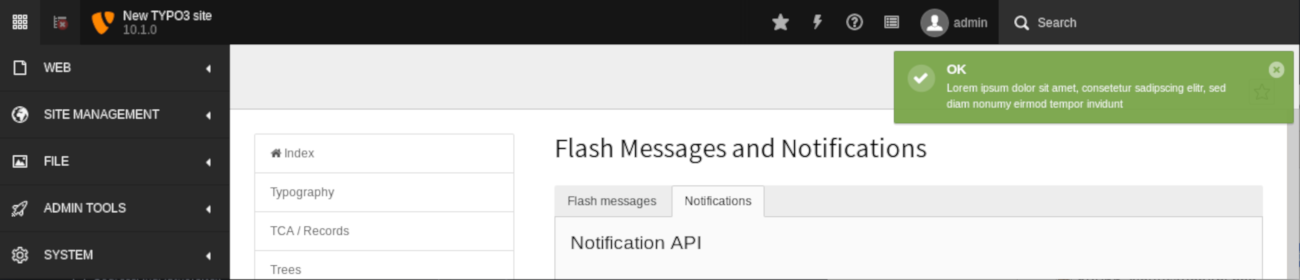
\includegraphics[width=0.90\linewidth]{ChangesForDevelopers/89066-NotificationApi.png}
%	\end{figure}
%
%\end{frame}

% ------------------------------------------------------------------------------
% Feature | 89061 | Introduce Notification Actions

\begin{frame}[fragile]
	\frametitle{Wijzigingen voor Ontwikkelaars}
	\framesubtitle{Berichtacties}

	\begin{itemize}
		\item JavaScript berichten in de backend ondersteunen nu actie(knoppen).
	\end{itemize}

	\begin{figure}
		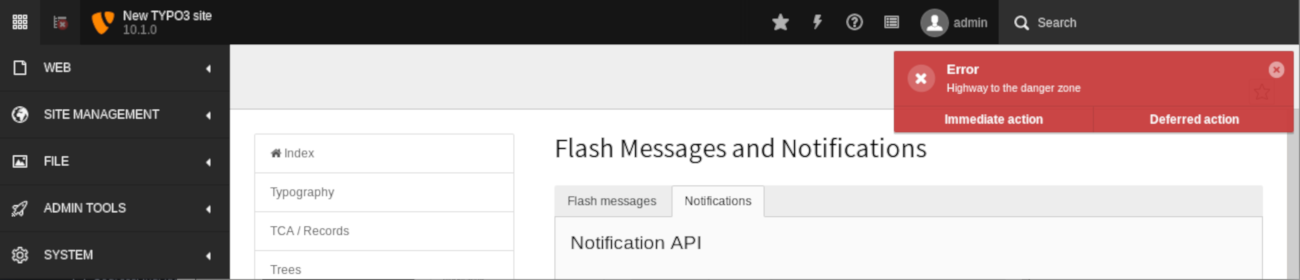
\includegraphics[width=0.90\linewidth]{ChangesForDevelopers/89061-NotificationActionsAndButtons.png}
	\end{figure}

\end{frame}

% ------------------------------------------------------------------------------
% Feature | 89244 | Broadcast Channels and Messaging

\begin{frame}[fragile]
	\frametitle{Wijzigingen voor Ontwikkelaars}
	\framesubtitle{Uitzendkanalen en berichtgeving (1)}

	% decrease font size for code listing
	\lstset{basicstyle=\tiny\ttfamily}

	\begin{itemize}
		\item Het is nu mogelijk om "uitzendberichten" met JavaScript te versturen en te ontvangen.
	\end{itemize}

	\vspace{-0.2cm}
	\begingroup
		\color{red}
			\begin{center}
				De API is voorlopig nog \textbf{intern}\newline
				en kan op elk moment wijzigen totdat het "stable" verklaard wordt.
			\end{center}
	\endgroup

	\begin{itemize}
		\item Voorbeeld voor het \textbf{versturen} van een bericht:

\begin{lstlisting}
require(['TYPO3/CMS/Backend/BroadcastService'], function (BroadcastService) {
  const payload = {
    componentName: 'my_extension',
    eventName: 'my_event',
    foo: 'bar'
  };
  BroadcastService.post(payload);
});
\end{lstlisting}

	\end{itemize}

\end{frame}

% ------------------------------------------------------------------------------
% Feature | 89244 | Broadcast Channels and Messaging

\begin{frame}[fragile]
	\frametitle{Wijzigingen voor Ontwikkelaars}
	\framesubtitle{Uitzendkanalen en berichtgeving (2)}

	% decrease font size for code listing
	\lstset{basicstyle=\tiny\ttfamily}

	\begin{itemize}
		\item Voorbeeld voor het \textbf{ontvangen} van het bericht:

\begin{lstlisting}
define([], function() {
  document.addEventListener('typo3:my_component:my_event', (e) => eventHandler(e.detail));
  function eventHandler(detail) {
    // output contains key 'foo' as the payload
    console.log(detail);
  }
});
\end{lstlisting}

		\item Zie \href{https://developer.mozilla.org/en-US/docs/Web/API/Broadcast_Channel_API}{developer.mozilla.org} voor meer details.

	\end{itemize}

\end{frame}

% ------------------------------------------------------------------------------
% Feature | 89018 | Provide implementation for PSR-17 HTTP Message Factories

\begin{frame}[fragile]
	\frametitle{Wijzigingen voor Ontwikkelaars}
	\framesubtitle{PSR-17 HTTP Message Factories}

	\begin{itemize}
		\item De \href{https://www.php-fig.org/psr/psr-17/}{PSR-17}
			HTTP Message Factories implementatie is toegevoegd.
		\item HTTP Message Factory koppelvlakken zouden als afhankelijkheden gebruikt worden voor
			request handlers of services die PSR-7 berichtobjecten aanmaken.
		\item PSR-17 bevat zes factory-koppelvlakken:

			\begin{itemize}\smaller
				\item \texttt{\textbackslash
					Psr\textbackslash
					Http\textbackslash
					Message\textbackslash
					RequestFactoryInterface}
				\item \texttt{\textbackslash
					Psr\textbackslash
					Http\textbackslash
					Message\textbackslash
					ResponseFactoryInterface}
				\item \texttt{\textbackslash
					Psr\textbackslash
					Http\textbackslash
					Message\textbackslash
					ServerRequestFactoryInterface}
				\item \texttt{\textbackslash
					Psr\textbackslash
					Http\textbackslash
					Message\textbackslash
					StreamFactoryInterface}
				\item \texttt{\textbackslash
					Psr\textbackslash
					Http\textbackslash
					Message\textbackslash
					UploadedFileFactoryInterface}
				\item \texttt{\textbackslash
					Psr\textbackslash
					Http\textbackslash
					Message\textbackslash
					UriFactoryInterface}

			\end{itemize}\normalsize

		\item Zie
			\href{https://docs.typo3.org/c/typo3/cms-core/master/en-us/Changelog/10.1/Feature-89018-ProvideImplementationForPSR-17HTTPMessageFactories.html}{documentatie}
			voor voorbeeldcode.

	\end{itemize}

\end{frame}

% ------------------------------------------------------------------------------
% Feature | 89216 | PSR-18 HTTP Client Implementation

\begin{frame}[fragile]
	\frametitle{Wijzigingen voor Ontwikkelaars}
	\framesubtitle{PSR-18 HTTP Client}

	\begin{itemize}
		\item De \href{https://www.php-fig.org/psr/psr-18/}{PSR-18}
			HTTP Client implementatie is toegevoegd.
		\item Hiermee kunnen ontwikkelaars HTTP request gebaseerd op PSR-7 berichtobjecten
			maken zonder af te hangen van een specifieke implementatie van een HTTP client.
		\item Het vervangt niet de bestaande \href{http://guzzlephp.org/}{Guzzle}
			functies maar biedt een meer generiek alternatief.
		\item PSR-18 bestaat uit een clientkoppelvlak en drie uitzonderingskoppelvlakken:

			\begin{itemize}\smaller
				\item \texttt{\textbackslash
					Psr\textbackslash
					Http\textbackslash
					Client\textbackslash
					ClientInterface}
				\item \texttt{\textbackslash
					Psr\textbackslash
					Http\textbackslash
					Client\textbackslash
					ClientExceptionInterface}
				\item \texttt{\textbackslash
					Psr\textbackslash
					Http\textbackslash
					Client\textbackslash
					NetworkExceptionInterface}
				\item \texttt{\textbackslash
					Psr\textbackslash
					Http\textbackslash
					Client\textbackslash
					RequestExceptionInterface}
			\end{itemize}\normalsize

		\item Zie
			\href{https://docs.typo3.org/c/typo3/cms-core/master/en-us/Changelog/10.1/Feature-89216-PSR-18HTTPClientImplementation.html}{documentatie}
			voor een codevoorbeeld.

	\end{itemize}

\end{frame}

% ------------------------------------------------------------------------------
% Feature | 88871 | Handle middleware handler in RequestFactory correctly

\begin{frame}[fragile]
	\frametitle{Wijzigingen voor Ontwikkelaars}
	\framesubtitle{RequestFactory Middleware Handler}

	% decrease font size for code listing
	\lstset{basicstyle=\tiny\ttfamily}

	\begin{itemize}
		\item Het is nu mogelijk om eigen middleware handlers als een array te definiëren.
		\item De RequestFactory bouwen een stapel handlers gebaseerd op de\newline
			\small
				\texttt{\$GLOBALS['TYPO3\_CONF\_VARS']['HTTP']['handler']}
			\normalsize
			array en injecteert het in de client.
		\item Bijvoorbeeld:

\begin{lstlisting}
use \TYPO3\CMS\Core\Utility\GeneralUtility;
use \Vendor\MyExtension\Middleware\Guzzle\CustomMiddleware;
use \Vendor\MyExtension\Middleware\Guzzle\SecondCustomMiddleware;

# Voeg eigen middleware toe aan de standaard Guzzle handler-stapel
$GLOBALS['TYPO3_CONF_VARS']['HTTP']['handler'][] =
  (GeneralUtility::makeInstance(CustomMiddleware::class))->handler();
$GLOBALS['TYPO3_CONF_VARS']['HTTP']['handler'][] =
  (GeneralUtility::makeInstance(SecondCustomMiddleware::class))->handler();
\end{lstlisting}

	\end{itemize}

\end{frame}

% ------------------------------------------------------------------------------
% Feature | 88602 | Allow registering additional file processors

\begin{frame}[fragile]
	\frametitle{Wijzigingen voor Ontwikkelaars}
	\framesubtitle{Eigen Bestandsprocessors}

	% decrease font size for code listing
	\lstset{basicstyle=\tiny\ttfamily}

	\begin{itemize}
		\item Ontwikkelaars kunnen nu eigen bestandsprocessors registreren.
		\item Voeg de volgende code toe aan het bestand \texttt{ext\_localconf.php}:

\begin{lstlisting}
$GLOBALS['TYPO3_CONF_VARS']['SYS']['fal']['processors']['ExampleImageProcessor'] = [
  'className' => \Vendor\MyExtension\Resource\Processing\ExampleImageProcessor::class,
  'before' => 'LocalImageProcessor',
];
\end{lstlisting}

		\item Voorbeeld van gebruik:

			\begin{itemize}
				\item een watermerk toevoegen aan afbeeldingen
				\item geüploade bestanden comprimeren in een ZIP-bestand
				\item bewerkte kopieën van afbeeldingen opslaan
				\item etc.
			\end{itemize}

	\end{itemize}

\end{frame}

% ------------------------------------------------------------------------------
% Feature | 88995 | Calling registerPlugin with vendor name

\begin{frame}[fragile]
	\frametitle{Wijzigingen voor Ontwikkelaars}
	\framesubtitle{Extbase en Fluid}

	% decrease font size for code listing
	\lstset{basicstyle=\smaller\ttfamily}

	\begin{itemize}
		\item Laat de vendor weg bij het registreren van plug-ins met\newline
			\smaller
				\texttt{\textbackslash
					TYPO3\textbackslash
					CMS\textbackslash
					Extbase\textbackslash
					Utility\textbackslash
					ExtensionUtility::registerPlugin()}
			\normalsize

		\item Bijv., gebruik "\texttt{Form}" in plaats van "\texttt{TYPO3.CMS.Form}"\newline
			\small(eerste parameter)\normalsize

\begin{lstlisting}
\TYPO3\CMS\Extbase\Utility\ExtensionUtility::registerPlugin(
  'Form',
  'Formframework',
  'Form',
  'content-form',
);
\end{lstlisting}

	\end{itemize}

\end{frame}

% ------------------------------------------------------------------------------
% Important | 89001 | TSFE->createHashBase
% Feature | 89150 | Add events before and after rollback of record history entries

\begin{frame}[fragile]
	\frametitle{Wijzigingen voor Ontwikkelaars}
	\framesubtitle{Diversen (1)}

	\begin{itemize}
		\item De \texttt{hashParameters} voor het berekenen van de hashBase zijn in de volgende klasse gewijzigde:\newline
			\small
				\texttt{TYPO3\textbackslash
					CMS\textbackslash
					Frontend\textbackslash
					Controller\textbackslash
					TypoScriptFrontendController}
			\normalsize

			\begin{itemize}
				\item \texttt{gr\_list} is vervangen door \texttt{groupIds}.
				\item \texttt{cHash} is vervangen door \texttt{dynamicArguments}.
				\item \texttt{domainStartPage} is vervangen door \texttt{site} (site identifier).
			\end{itemize}

		\item Twee nieuwe gebeurtenissen worden verstuurd als records teruggedraaid worden:

			\begin{itemize}\smaller
				\item \texttt{TYPO3\textbackslash
					CMS\textbackslash
					Backend\textbackslash
					History\textbackslash
					Event\textbackslash
					BeforeHistoryRollbackStartEvent}
				\item \texttt{TYPO3\textbackslash
					CMS\textbackslash
					Backend\textbackslash
					History\textbackslash
					Event\textbackslash
					AfterHistoryRollbackFinishedEvent}
			\end{itemize}\normalsize

	\end{itemize}

\end{frame}

% ------------------------------------------------------------------------------
% Feature | 88805 | Add type to TYPO3/CMS/Core/Database/Query/QueryBuilder::set()

\begin{frame}[fragile]
	\frametitle{Wijzigingen voor Ontwikkelaars}
	\framesubtitle{Diversen (2)}

	\begin{itemize}
		\item Methode \texttt{set()} van de querybouwer kent nu een 4e parameter
			om het type van de parameter met naam te specificeren:\newline
			\small
				\texttt{TYPO3\textbackslash
					CMS\textbackslash
					Core\textbackslash
					Database\textbackslash
					Query\textbackslash
					QueryBuilder::set()}
			\normalsize\newline
			\vspace{0.2cm}
			(de standaard is \texttt{\textbackslash PDO::PARAM\_STR})

	\end{itemize}

\end{frame}

% ------------------------------------------------------------------------------
